\documentclass[12pt]{beamer}
\usepackage{listings}
\beamertemplatenavigationsymbolsempty
\AtBeginSection[]
{
    \begin{frame}
    \frametitle{Table of Contents}
    \tableofcontents[currentsection]
    \end{frame}
}
\lstset{language=C++, basicstyle=\footnotesize}
\setlength{\tabcolsep}{10pt}

\title{Graph traversal}
\subtitle{DFS, BFS, applications}
\author{beOI Training}
\institute{
\includegraphics[height=12em]{img/beoi-logo}}

\begin{document}

\frame{\titlepage}

\section{DFS and BFS}

\begin{frame}
\frametitle{Depth-first principle}
\begin{itemize}
\item Go in depth, backtrack when stuck
\item Visit everything before switching
\end{itemize}
\begin{figure}
\centering
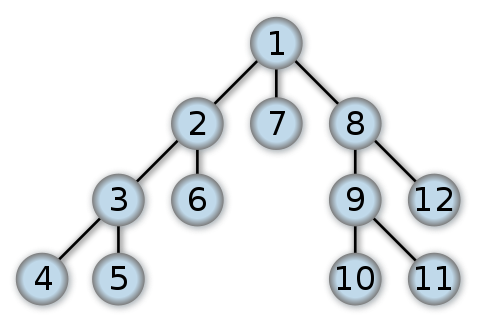
\includegraphics[width=.5\linewidth]{img/dfs-tree}
\end{figure}
\end{frame}

\begin{frame}
\frametitle{DFS example}
Do not visit a node twice!
\begin{figure}
\centering
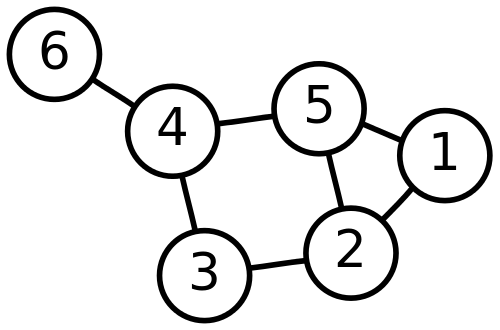
\includegraphics[width=.5\linewidth]{img/6n-graph}
\end{figure}
\[ \mathbf{1} \to \mathbf{2} \to \mathbf{3} \to \mathbf{4} \to \mathbf{5} \to 4 \to \mathbf{6} \to 4 \to 3 \to 2 \to 1 \]
\end{frame}

\begin{frame}[fragile]
\frametitle{DFS recursive implementation}
\begin{lstlisting}
vector<int> neigh[MAXN];
bitset<MAXN> visited;

void dfs(int u)
{
    if (visited[u])
        return;
    visited[u] = true;

    for (int i = 0; i < (int) neigh[u].size(); i++)
        dfs(neigh[u][i]);
}
\end{lstlisting}
\end{frame}

\begin{frame}
\frametitle{DFS visit order}
\begin{itemize}
\item Always travels locally: parent $\to$ child $\to$ parent
\item The last discovered are the first visited $\Rightarrow$ we can also use a \emph{Last In First Out} structure (stack)
\end{itemize}
\begin{figure}
\centering
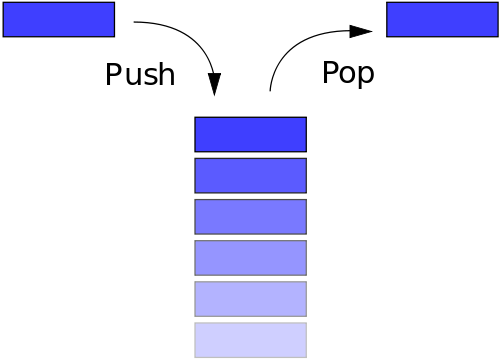
\includegraphics[width=.5\linewidth]{img/stack}
\end{figure}
\end{frame}

\begin{frame}[fragile]
\frametitle{DFS stack implementation}
\begin{lstlisting}
stack<int> st;
st.push(start);

while (!st.empty())
{
    int u = st.top();
    st.pop();
    
    for (int i = 0; i < (int) neigh[u].size(); i++)
    {
        int v = neigh[u][i];
        if (!visited[v])
        {
            visited[v] = true;
            st.push(v);
        }
    }
}
\end{lstlisting}
\end{frame}

\begin{frame}
\frametitle{Breadth-first principle}
\begin{itemize}
\item Go layer by layer
\item Visit the closest nodes first
\end{itemize}
\begin{figure}
\centering
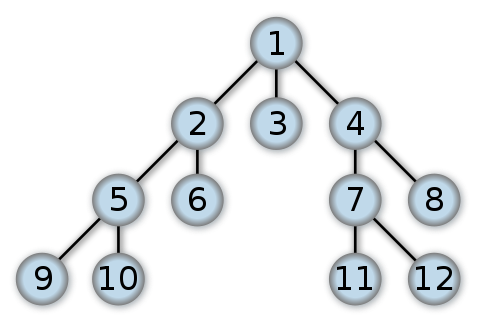
\includegraphics[width=.5\linewidth]{img/bfs-tree}
\end{figure}
\end{frame}

\begin{frame}
\frametitle{BFS example}
\begin{figure}
\centering
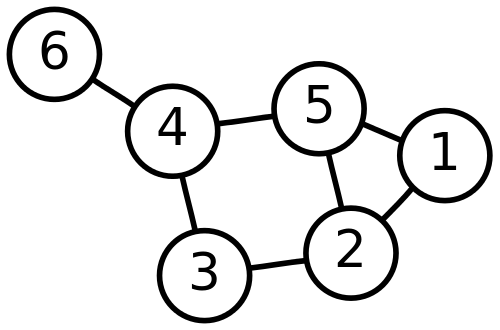
\includegraphics[width=.5\linewidth]{img/6n-graph}
\end{figure}
\[ 1 \to 2 \to 5 \to 3 \to 4 \to 6 \]
\end{frame}

\begin{frame}
\frametitle{BFS visit order}
The first discovered are the first visited $\Rightarrow$ we can use a \emph{First In First Out} structure (queue)
\begin{figure}
\centering
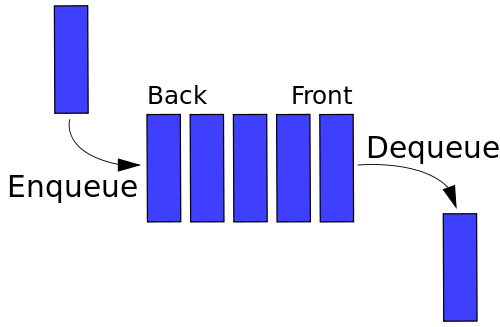
\includegraphics[width=.6\linewidth]{img/queue}
\end{figure}
\end{frame}

\begin{frame}[fragile]
\frametitle{BFS implementation}
\begin{lstlisting}
queue<int> q; // different
q.push(start);

while (!q.empty())
{
    int u = q.front(); // different
    q.pop();
    
    for (int i = 0; i < (int) neigh[u].size(); i++)
    {
        int v = neigh[u][i];
        if (!visited[v])
        {
            visited[v] = true;
            q.push(v);
        }
    }
}
\end{lstlisting}
\end{frame}

\begin{frame}
\frametitle{BFS for shortest path}
BFS traverses graph with nondecreasing distance!
\begin{itemize}
\item Add two tables \texttt{dist[]} and \texttt{parent[]}
\item When adding to queue:
    \begin{itemize}
    \item \lstinline[basicstyle=\normalsize]{dist[v] = dist[u] + 1}
    \item \lstinline[basicstyle=\normalsize]{parent[v] = u}
    \end{itemize}
\item Trace path back using \texttt{parent[]}
\end{itemize}
\end{frame}

\begin{frame}
\frametitle{Comparison}
Complexity: both $O(V+E)$.

~

How to choose:
\begin{itemize}
\item If distance / shortest path necessary $\Rightarrow$ BFS
\item Otherwise $\Rightarrow$ DFS (shorter)
\end{itemize}
\end{frame}

\section{Connected components}

\begin{frame}
\frametitle{Connected components}
\begin{itemize}
\item On \textbf{undirected graphs}, ``$u$ connected to $v$'' is an equivalence relation
\item So it forms a partition of the vertices
\end{itemize}
\begin{figure}
\centering
\begin{tabular}{cc}
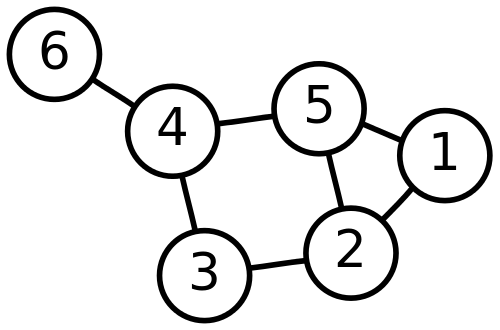
\includegraphics[width=0.4\linewidth]{img/6n-graph}
& 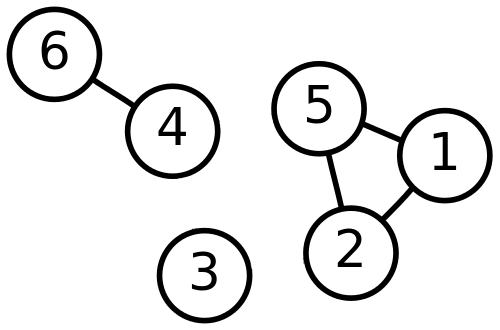
\includegraphics[width=0.4\linewidth]{img/6n-3comp} \\
1 connected component & 3 connected components
\end{tabular}
\end{figure}
\end{frame}

\begin{frame}[fragile]
\frametitle{Finding connected components}
One run of DFS/BFS visits a whole component!
\begin{itemize}
\item Go through nodes and check if visited
\item In \texttt{dfs()}, store nodes in a vector
\end{itemize}
\begin{lstlisting}
for (int i = 0; i < n; i++)
{
    if (!visited[i]) // new CC
    {
        vector<int> cc;
        dfs(i, &cc); // adds nodes to cc
        // process cc
    }
}
\end{lstlisting}
\end{frame}

\section{Topological sort}

\begin{frame}
\frametitle{Directed acyclic graphs}
Directed graphs without cycles
\begin{figure}
\centering
\begin{tabular}{cc}
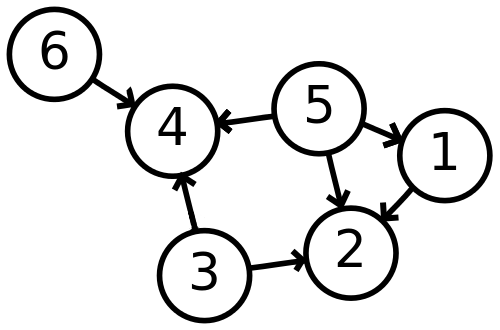
\includegraphics[width=0.4\linewidth]{img/6n-dag}
& 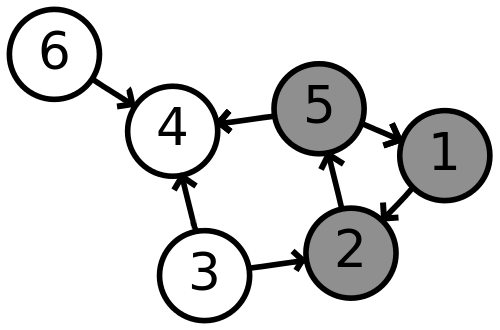
\includegraphics[width=0.4\linewidth]{img/6n-not-dag} \\
DAG & not DAG
\end{tabular}
\end{figure}
\end{frame}

\begin{frame}
\frametitle{Topological sort}
\begin{itemize}
\item There are no cycles, so we can order the nodes so that edge $u \to v \Rightarrow  u$ before $v$
\item Example: course prerequisites, how to take them all in order
\item Not unique: $\{3,5,6,4,1,2\}, \{5,3,1,6,2,4\},\ldots$
\end{itemize}
\begin{figure}
\centering
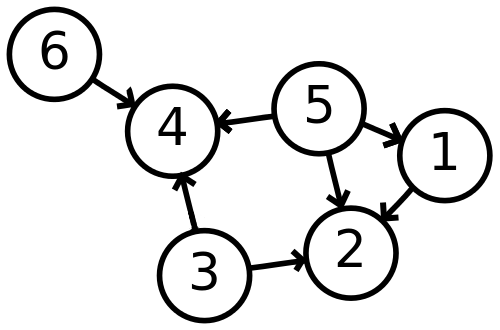
\includegraphics[width=.5\linewidth]{img/6n-dag}
\end{figure}
\end{frame}

\begin{frame}
\frametitle{Toposort with zero in-degree}
If $u$ does not have edges pointing to it, it can go first!
\begin{itemize}
\item Start at nodes with $\mathsf{deg}_\mathsf{in} = 0$
\item Remove edges as we find them
\item Continue until no node is left
\end{itemize}
\end{frame}

\begin{frame}[fragile]
\frametitle{Zero in-degree implementation}
\begin{lstlisting}
int in_degree[MAXN];  // pre-filled
queue<int> zero_in;   // pre-filled
vector<int> toposort;

while (!zero_in.empty())
{
    int u = zero_in.front();
    zero_in.pop();
    toposort.push_back(u);
    
    for (int i = 0; i < (int) neigh[u].size(); i++)
    {
        int v = neigh[u][i];
        in_degree[v]--;
        if (in_degree[v] == 0)
            zero_in.push(v);
    }
}
\end{lstlisting}
\end{frame}

\begin{frame}
\frametitle{Toposort with DFS}
Use DFS to build the toposort backwards
\begin{itemize}
\item Call \texttt{dfs()} on every node
\item Add a node \emph{after} recursing
\end{itemize}
Thus every node is
\begin{itemize}
\item after its children in the \emph{backward} toposort
\item before its children in the \emph{forward} toposort
\end{itemize}
\end{frame}

\begin{frame}[fragile]
\frametitle{Toposort DFS implementation}
\begin{lstlisting}
int dfs(int u, vector<int> *toposort)
{
    if (visited[u]) return;
    visited[u] = true;
    // recurse as usual...
    toposort->push_back(u);
}

vector<int> toposort;
for (int i = 0; i < n; i++)
    dfs(i, &toposort); // no need to check visited[i]

for (int i = n-1; i >= 0; i--)
    // use toposort[i]
\end{lstlisting}
\end{frame}

\begin{frame}
\frametitle{Comparison}
Complexity: both $O(V+E)$

~

Use the zero in-degree method only if needed:
\begin{itemize}
\item Additional conditions on the order
\item Enumerate all possible toposorts
\end{itemize}
\end{frame}

\section{Bipartite check}

\begin{frame}
\frametitle{Bipartite graphs}
\begin{itemize}
\item Can be split in two without internal edges
\item Equivalent: no odd-length cycle
\end{itemize}
\begin{figure}
\centering
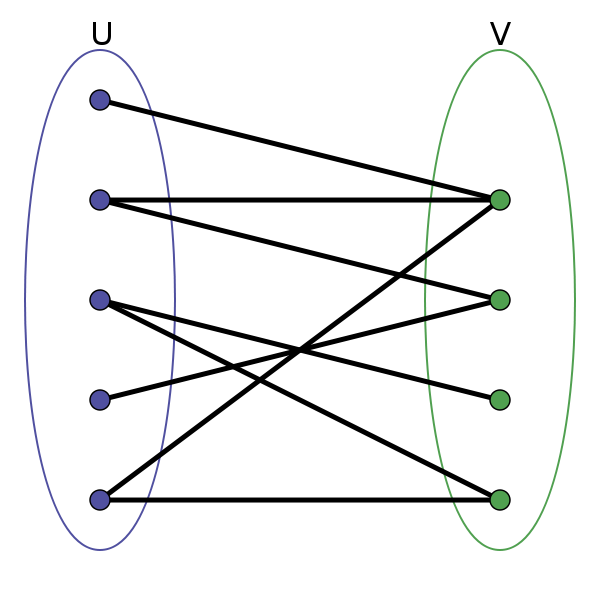
\includegraphics[width=0.5\linewidth]{img/bipartite}
\end{figure}
\end{frame}

\begin{frame}
\frametitle{Bipartite examples}
\begin{figure}
\centering
\begin{tabular}{cc}
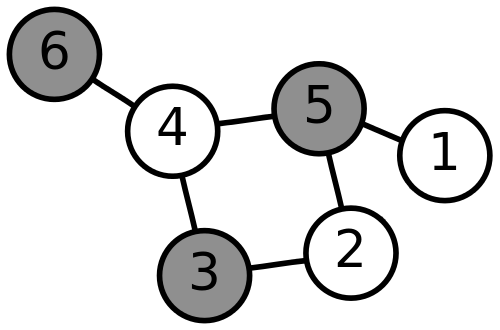
\includegraphics[width=0.4\linewidth]{img/6n-bipartite}
& 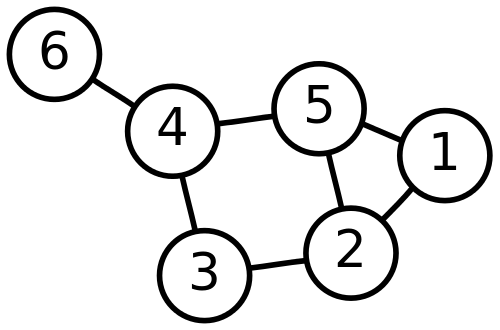
\includegraphics[width=0.4\linewidth]{img/6n-graph} \\
bipartite & not bipartite
\end{tabular}
\end{figure}
\end{frame}

\begin{frame}
\frametitle{Bipartite check with DFS/BFS}
Put an arbitrary node $u$ on the left then traverse the graph:
\begin{itemize}
\item If $v$ is on the left, put all its neighbors on the right
\item If $v$ is on the right, put all its neighbors on the left
\item Continue until conflict or finished
\end{itemize}
Note: $v$ on left $\Leftrightarrow \mathsf{dist}(u,v)$ even
\end{frame}

\begin{frame}
\frametitle{Bipartite check correctness}
$G$ is not bipartite $\Leftrightarrow$ the assignment fails
\begin{itemize}
\item If $G$ is not bipartite the assignment will clearly fail
\item If there is a conflict between $u$ and $v$ adjacent
    \begin{itemize}
    \item Let $p$ be their common parent in the DFS
    \item $\mathsf{dist}(p,u)$ and $\mathsf{dist}(p,v)$ have the same parity
    \item Cycle $p-u-v$ has odd length $\mathsf{dist}(p,u) + 1 + \mathsf{dist}(p,v)$
    \item Thus $G$ is not bipartite
    \end{itemize}
\end{itemize}
\end{frame}

\begin{frame}[fragile]
\frametitle{Bipartite check implementation}
\begin{lstlisting}
int color[MAXN];

bool dfs(int u)
{
    for (int i = 0; i < (int) neigh[u].size(); i++)
    {
        int v = neigh[u][i];
        if (color[v] == -1) // unassigned
        {
            color[v] = !color[u];
            if (!dfs(v))
                return false;
        }
        else if (color[u] == color[v]) // conflict
            return false;
    }
    return true;
}
\end{lstlisting}
\end{frame}

\section{Kosaraju SCC}

\begin{frame}
\frametitle{Strongly connected components}
Nodes $u,v$ in same SCC $\Leftrightarrow$ path $u \to v$ \textbf{and} path $v \to u$
\begin{figure}
\centering
\begin{tabular}{c}
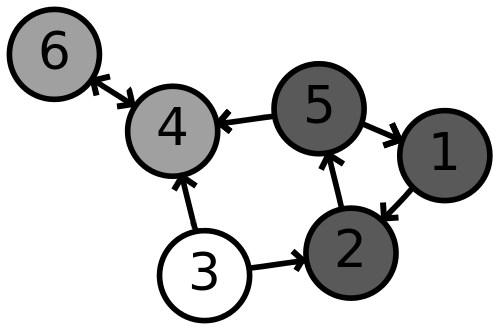
\includegraphics[width=0.5\linewidth]{img/6n-scc} \\
3 strongly connected components
\end{tabular}
\end{figure}
\end{frame}

\begin{frame}
\frametitle{Contracted graph}
\begin{itemize}
\item If we contract the SCCs into one node, a DAG appears
\item This is because all cycles have been contracted
\item Useful for DP (as we will see later)
\end{itemize}
\begin{figure}
\centering
\begin{tabular}{cc}
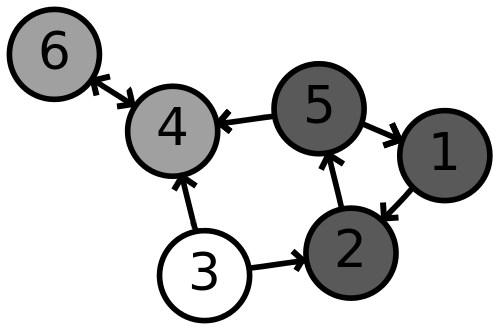
\includegraphics[width=0.4\linewidth]{img/6n-scc}
& 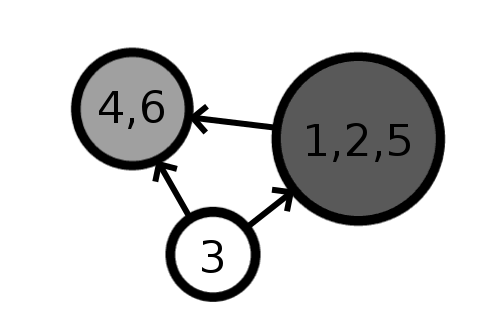
\includegraphics[width=0.4\linewidth]{img/6n-contracted} \\
original & contracted
\end{tabular}
\end{figure}
\end{frame}

\begin{frame}
\frametitle{Kosaraju's algorithm}
\begin{itemize}
\item Run the DFS toposort algorithm on $G$
\item Use that order and flood with the transpose of $G$
\end{itemize}
\begin{figure}
\centering
\begin{tabular}{cc}
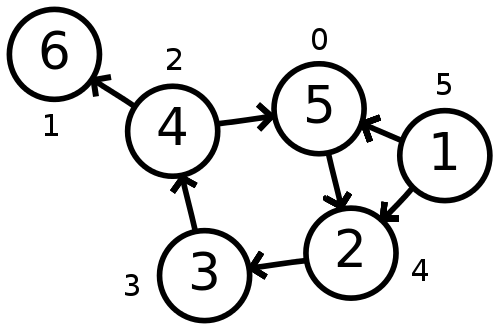
\includegraphics[width=0.4\linewidth]{img/6n-kosa1}
& 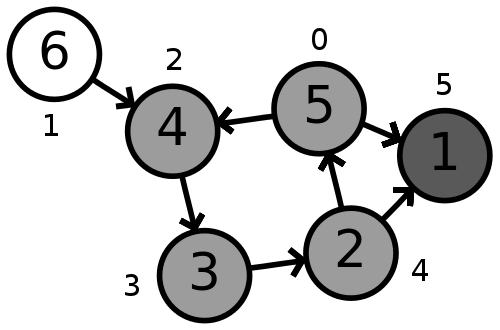
\includegraphics[width=0.4\linewidth]{img/6n-kosa2} \\
raw toposort order & flood with decreasing index
\end{tabular}
\end{figure}
\end{frame}

\begin{frame}[fragile]
\frametitle{Kosaraju implementation}
\begin{lstlisting}
void dfs(int u, vector<int> neigh[], vector<int> *st)
{
    // ... (use neigh[] to flood)
    st->push_back(u);
}

vector<int> toposort; // not valid toposort!
for (int i = 0; i < n; i++)
    dfs(i, neigh, &toposort);
visited.reset();
for (int i = n-1; i >= 0; i--)
{
    if (!visited[toposort[i]])
    {
        vector<int> scc;
        dfs(toposort[i], neighT, &scc);
    }
}
\end{lstlisting}
\end{frame}

\begin{frame}
\frametitle{Source of figures}
\begin{itemize}
\item \url{https://en.wikipedia.org/wiki/File:6n-graf.svg}
\item \url{http://en.wikipedia.org/wiki/File:Depth-first-tree.svg}
\item \url{http://en.wikipedia.org/wiki/File:Data_stack.svg}
\item \url{http://en.wikipedia.org/wiki/File:Breadth-first-tree.svg}
\item \url{http://en.wikipedia.org/wiki/File:Data_Queue.svg}
\item \url{https://commons.wikimedia.org/wiki/File:Simple-bipartite-graph.svg}
\end{itemize}
\end{frame}

\end{document}
